\documentclass{article}

\usepackage{fancyhdr}
\usepackage{graphicx}
\graphicspath{{}}


\title{BPP Exercise 2 - The Very Basics}
\author{A. Hain, M. Nipshagen}
\date{16.04.2018, 8:00}

\makeatletter
\let\thetitle\@title
\let\theauthor\@author
\let\thedate\@date
\makeatother

\pagestyle{fancy}
\fancyhf{}
\fancyhead[L]{\thetitle}
\fancyhead[C]{}
\fancyhead[R]{\theauthor}
\renewcommand{\headrulewidth}{0.4pt} %obere Trennlinie
\fancyfoot[L]{Due: \thedate}
\fancyfoot[R]{\thepage} %Seitennummer
\renewcommand{\footrulewidth}{0.4pt}
\begin{document}

The deadline for this exercise sheet is \textbf{Monday, \thedate.}
%
%\section*{Introductory Words}
%In case we have some information that doesn't directly concern the current exercises.
%
\section{Variable Types}
Assume you're enrolled in a Psychology class.
Your final grade is dependent on your performance in homework, a midterm exam and an experiment as a final project.\\
\textit{Note:} Save your answers for this task in a simple text file.

\subsection{}
You just wrote the midterm and after correcting, your professor thinks it might be handy
to have the exam results for each student digitally accessible. Which variable types would you use
for variables to save the following things in? Explain your answers.
\begin{enumerate}
\item the student's name
\item the student's matriculation number
\item the student's exam grade
\item if the student passed the exam or not
\end{enumerate}

\subsection{}
Fast foward some time, you need to conduct the experiment.
Something something still need to come up with some sort of experiment

\section{Some Calculations [insert better task name maybe]}
In this task, you will have to write two small Python programs. Please save each
of them in a separate file.

\subsection{-}
After you completed your Psychology class, your professor now wants to determine your final grade.
It is composed of your homework grade by 20\%, your midterm grade by 30\% and your final
project grade by 50\%.\\
Write a Python script which will calculate the final grade out of those three grades
and print the result. Try to use suitable names for your variables and test your program with
a few different values.

\subsection{Also needs title}
After passing the class with -of course- 1.0, you want to treat yourself by baking
a chocolate cake. You find a nice recipe for the batter online. The quantities of
the ingredients are perfect to make one cake in a circular cake mould with a diameter
of 28cm and a height of 8cm. However, you only have a cake mould with a diameter of 24cm and a height of 6.5cm.\\
Write a script that determines by which factor you need to multiply the cake ingredients to
make the perfect amount of batter for your smaller cake mould and prints the result.\\What is the factor if you only
have a cake mould with a 20cm diameter/6cm height? Or 18cm diameter/6cm height?\\

\begin{center}
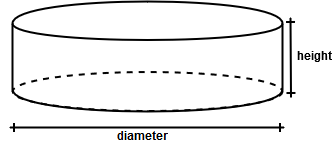
\includegraphics[scale=0.6]{Ex_2_Cake}
\end{center}

\end{document}
